\documentclass[12pt,titlepage]{article}



%PACKAGES
\usepackage{titling}
\newcommand{\subtitle}[1]{%
	\posttitle{%
		\par\end{center}
	\begin{center}\large#1\end{center}
	\vskip0.5em}%
}

\usepackage[ngerman]{babel}
% Verhindert die Formatierung von Hyperlinks
\usepackage[hidelinks]{hyperref}
% Ermöglicht die Einbindung von Bildern
\usepackage{graphicx}
% Ermöglicht vereinfachtes Zitieren
\usepackage{apacite}
% Für bessere Beschriftungen
\usepackage{caption}
% Für die Beschriftung von Unterbilder/Tabellen
\usepackage{subcaption}
\usepackage[utf8]{inputenc}

\usepackage{color}
\usepackage[a4paper,lmargin={3cm},rmargin={3cm},
tmargin={2.5cm},bmargin = {2.5cm}]{geometry}
\usepackage{amssymb}
\usepackage{amsthm}
\usepackage{titleref}

% Neue Referenzarten
\newcommand{\imgref}[1]{{siehe \textit{Abbildung \ref{#1}}}}
\newcommand{\imgrefplain}[1]{{\textit{Abbildung \ref{#1}}}}
\newcommand{\secref}[1]{{\textit{Kapitel \ref{#1}, Seite \pageref{#1}}}}
\newcommand{\secrefplain}[1]{{\textit{\ref{#1}: \nameref{#1}, Seite \pageref{#1}}}}
\newcommand{\tblref}[1]{{siehe \textit{Tabelle \ref{#1}: \nameref{#1}}}}
\newcommand{\tblrefplain}[1]{{\textit{Tabelle \ref{#1}: \nameref{#1}}}}
\newcommand{\calcref}[1]{{siehe \textit{Berechnung \ref{#1}, Seite \pageref{#1}}}}
\newcommand{\calcrefplain}[1]{{\textit{\ref{#1}, Seite \pageref{#1}}}}
\newcommand{\appref}[1]{{\textit{Anhang \ref{#1}}}}


\setlength{\parindent}{0pt}



\begin{document}



%TITELSEITE

\title{Projektdokumentation Datenbanksysteme}
\subtitle{\textbf{\Large{Erfolgsfaktoren auf YouTube}}}
\author{Adrian Franz Willi\\
	Frederico Fischer\\
Nico Iseli\\
Rahul Pucadyil\\ \\ \\}


\date{Abgabedatum: 25. Juni 2020\\
	Dozent: Prof. Dr. Michael Kaufmann\\
	Eingereicht im Rahmen des Studiengangs: Informatik  \linebreak \linebreak \linebreak \linebreak \linebreak \linebreak \linebreak \linebreak \linebreak \linebreak
\textbf{Hochschule Luzern}\\
Departement Informatik}



\thispagestyle{empty}
\maketitle





%INHALTSVERZEICHNIS
\tableofcontents
\newpage


%ABBILDUNGSVERZEICHNIS
\addcontentsline{toc}{section}{Abbildungsverzeichnis}
\listoffigures
\newpage



%TABELLENVERZEICHNIS
\addcontentsline{toc}{section}{Tabellenverzeichnis}
\listoftables
\newpage



%EINLEITUNG
\section{Einleitung}
\subsection{Ausgangslage und Problemstellung}
%Was ist der Kontext, warum ist das Projekt relevant, und worum geht es?
Im Rahmen des Moduls Datenbanksysteme wird den Studierenden des Studiengangs Informatik der Hochschule Luzern die Aufgabe gestellt, ein Projekt durchzuführen, das passend zu den theoretischen Inputs ebenfalls die Praxis abdeckt. Die Studierenden bilden dafür Projektgruppen und definieren dabei einen Use-Case, den sie behandeln möchten. In der Themenwahl sind sie frei.\\
\\
Das Projekt ist insofern relevant, als dass es Theorie sowie Praxis kombiniert. Ferner haben die Studierenden die Möglichkeit, sich in einer spezifischen Domäne zu spezialisieren (Technologie, Datenbanken etc.). 
\subsection{Aufbau und Methodik}
Der Aufbau erfolgt anhand der Vorlesungen. Daher sollen die wöchentlichen Inputs jeweils in die Arbeit einfliessen, damit die Aufgaben über das Semester verteilt werden. 

\subsection{Zielsetzung}
Ziel des Projekts ist es, dass sich die Studierenden in einer spezifischen Datenbanktechnologie vertiefen und dadurch neben den Inputs durch die Vorlesungen von weiterem Wissenserwerb profitieren. Ein weiterer Anspruch an das Projekt ist das Umsetzen eines sinnvollen Use Cases. Dadurch wird neben den Technologieaspekten auch der wirtschaftliche und wissenschaftliche Nutzen abgedeckt.
\newpage



%DATENMANAGEMENT
\section{Datenmanagement}
\subsection{Datennutzung}
\subsubsection{Use Case}
%Für welche Anwendung (Use Case) wird die Datenbank in ihrem Projekt eingesetzt? 
Für das vorliegende Projekt hat sich das Projektteam dazu entschieden, Daten von Youtube-Videos zu analysieren. Youtube hat seit ihrer Gründung im Jahr 2005 kontinuierlich an Popularität gewonnen und ermöglicht heutzutage sogar, die Plattform als Vollzeitbeschäftigung zu nutzen. Durch die zunehmende Bedeutung von Werbekampagnen und \glqq Affiliate Marketing\grqq\, etabliert sich der Beruf \glqq Youtuber\grqq\, und \glqq Influencer\grqq\, immer wie mehr als Berufsbezeichnung. Für Leute, die einem solchen Beruf nachgehen möchten, ist es zunächst wichtig, Erfolgsfaktoren zu erkennen und ihre Community stets auszubauen. Die Plattform ist jedoch nicht nur für Erwerbstätige in diesem Bereich interessant. Aufmerksamkeit oder Informationsverbreitung sind weitere treibende Faktoren, die Plattform zu nutzen. Auch für diese Anspruchsgruppe ist das Wissen über erfolgsversprechende Aspekte wichtig.\\
\\
Erfolg ist sehr individuell interpretierbar. Für die einen sind viele Likes wichtig, andere wollen eine möglichst hohe Anzahl an Views und wiederum andere möchten sich mit ihrer Konkurrenz vergleichen. Daher hat das Projekt zum Ziel, über eine Webseite möglichst viele Anfragen zu ermöglichen, so dass der Youtuber (also der Kunde) seinen Account optimal analysieren kann. Die Auswertungen sollen im Anschluss graphisch dargestellt werden, so dass diese auch für den Laien verständlich sind.\\
\\
Der genutzte Datensatz ist auf Kaggle unter dem Namen \glqq Trending YouTube Video Statistics\grqq\, verfügbar \shortcite{dataset}. Kaggle ist eine Online-Community, die sich an Datenwissenschaftler richtet und eine Menge an freien Daten zur Verfügung stellt.

\subsubsection{Entscheidungsgrundlage}
%Welche Entscheidung soll wie unterstützt werden?
Wie bereits erwähnt, sind Ziele und der Erfolg auf Youtube sehr individuell zu betrachten. Eine hohe Anzahl Views, viele Like oder eine umfangreiche Diskussion mit der Community (Kommentare) sind nur einige Beispiele davon. Die vorliegende Arbeit hat daher zum Ziel, dass jeder Youtuber seinen Account analysieren kann und dabei die Möglichkeit hat, die für ihn wichtigen Zahlen zu beurteilen. Damit kann er sich mit wenigen Mausklicks sofort einordnen und abschätzen, wie es um seine Erfolgschancen steht. 

\newpage

\subsection{Datenarchitektur}
%Welche Daten (Klassen, Attribute) brauchen Sie für Ihren Use Case? 
Um das Ziel des Use Cases zu erreichen, wurden folgende Daten verwendet:
\begin{itemize}
\item Video
\begin{itemize}
\item ID
\item Titel
\item Veröffentlicht (Datum)
\item Trends erreicht (Datum)
\item Herkunft (Land)
\end{itemize}
\item Channel
\begin{itemize}
\item ID
\item Titel
\end{itemize}
\item Interaktionen
\begin{itemize}
\item Likes / Dislikes
\item Views
\item Anzahl Kommentare
\item Ratings
\end{itemize}
\item Kategorien
\begin{itemize}
\item ID
\item Name
\end{itemize}
\end{itemize}

Die Eigenschaften dieser Daten werden im Kapitel \glqq Datenmodellierung\grqq\, (vgl. Abschnitt \ref{Datenmodellierung} auf Seite \pageref{Datenmodellierung}) genauer erläutert. Diese Daten wurden von Mitchell Jolly auf Kaggle \shortcite{dataset} bezogen. Auf die Herkunft dieser Daten wird im Kapitel \glqq Quelle und Import\grqq\, (vgl. Abschnitt \ref{Quelle und Import} auf Seite \pageref{Quelle und Import}) genauer eingegangen.
\newpage

\subsection{Datenadministration}
%Wer ist die Zielgruppe der Datenauswertung? Wer erhält wie Zugriff? 
Mit dem Use Case sollen Personen angesprochen werden, die Youtube erfolgreich nutzen möchten. Die Datenauswertung soll ermöglichen, den eigenen Account analysieren zu können. Die Ergebnisse werden über ein Website zur Verfügung gestellt, die auf Anfrage individuelle Resultate liefert. Die Resultate sind somit für alle zugänglich. 

\subsection{Datentechnik}
%Um welche Datenbanktechnologie handelt es sich? • Wie wird die Datenmigration umgesetzt?
Als Datentechnik wurde aus Interessensgründen entschieden, eine NoSQL-Technik zu verwenden. Hierfür ist MongoDB angedacht, die Daten im JSON-Format verwaltet. Grund hierfür ist, dass MongoDB eine weit verbreitete NoSQL-Technologie ist und somit eine grosse Community aufweist. Dadurch lässt sich bei Problemen schneller eine sichere Quelle finden. Für den Server wird auf die Ressourcen vom Enterpriselab zurückgegriffen. Dafür wurde eine Virtuelle Maschine mit Ubuntu reserviert. Da die Ressource extern bezogen wird, ist die Katastrophenvorsorge sowie die Replikation durch das Enterpriselab sichergestellt.
Die Daten werden im CSV-Format bezogen.

\subsection{Übersicht Architektur des Projektes}
Um die nachfolgenden Erläuterung besser im Kontext des vorliegenden Projektes zu verstehen, werden hier die verwendeten Technologien sowie die gesamte Architektur (vgl. Abbildung \ref{img: Architektur des Projektes} auf Seite \pageref{img: Architektur des Projektes}) erläutert. Die Architektur lässt sich in drei Schichten (Daten, Logik und Präsentation) unterteilen. In der Datenschicht wird, wie bereits erwähnt, MongoDB verwendet, um die Daten zu speichern. In der darüberliegenden Logikschicht erfolgen die Abfragen sowie deren Verarbeitung. Die gesamte Logik ist in der Programmiersprache Python geschrieben. Damit die User Abfragen machen können, wird mit Hilfe des Webframeworks Flask eine Website generiert. Die Webseite selbst nutzt die gängigen Webtechnologien wie HTML, CSS und JavaScript.
\begin{figure}
	\centering
	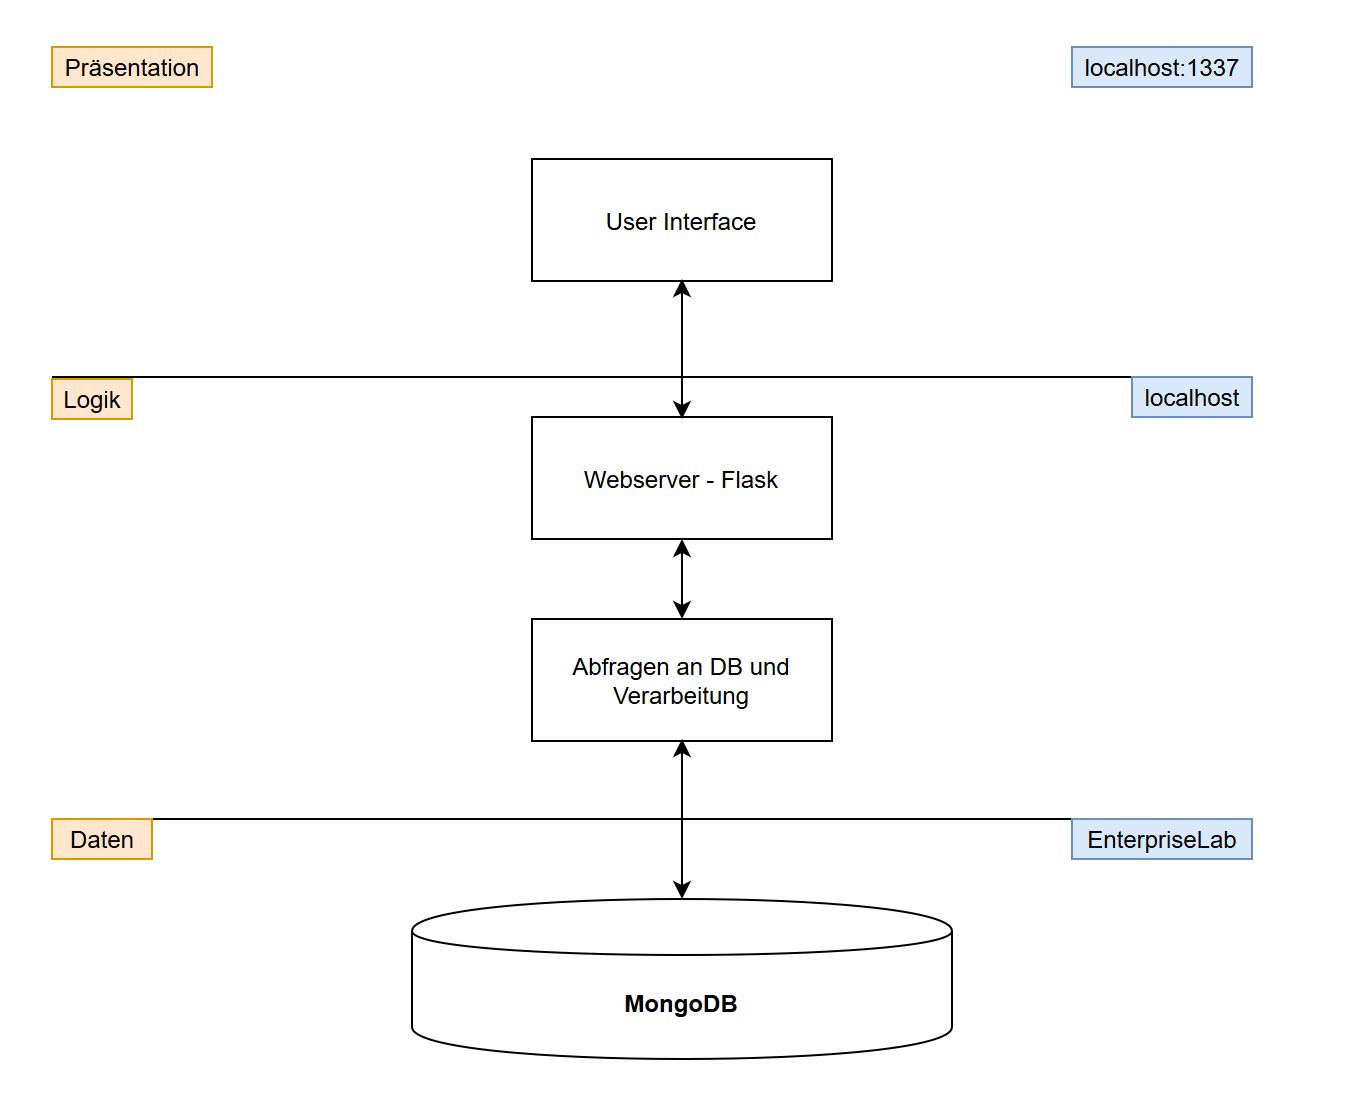
\includegraphics[width=16cm]{IMG/Architektur.JPG}
	\caption[Architektur des Projektes]{Architektur des Projektes,\\ Quelle: Autoren}
	\label{img: Architektur des Projektes}
\end{figure}
\newpage



%DATENMODELLIERUNG
\section{Datenmodellierung} \label{Datenmodellierung}
\subsection{Datenmodell}
Wie bereits erwähnt, wird im vorliegenden Projekt auf eine NoSql-Lösung mit MongoDB zurückgegriffen. Die Verwaltung der Daten erfolgt daher im JSON-Format. Grundsätzlich umfasst das vorliegende Projekt zwei Collections (vgl. Abbildung \ref{img: Modellierung Collections} auf Seite \pageref{img: Modellierung Collections}). Das ist zum einen \glqq videos\grqq\, und zum anderen \glqq categories\grqq. Die Collection \glqq videos\grqq\, beinhaltet entsprechende Daten von Trendvideos, während \glqq categories\grqq\, die von YouTube vorgegebenen Kategorien enthält. Da die Collection \glqq videos\grqq\, aus sehr vielen Attributen besteht, wurde entschieden, diese innerhalb der JSON-Struktur zu verschachteln. Deshalb sind nun zusätzlich die Objekte \glqq channel\grqq, \glqq settings\grqq\, und \glqq interactions\grqq\, der Collection \glqq videos\grqq\, untergeordnet. Dadurch erhält das JSON-Dokument eine bessere Struktur.

\begin{figure}[h]
\centering
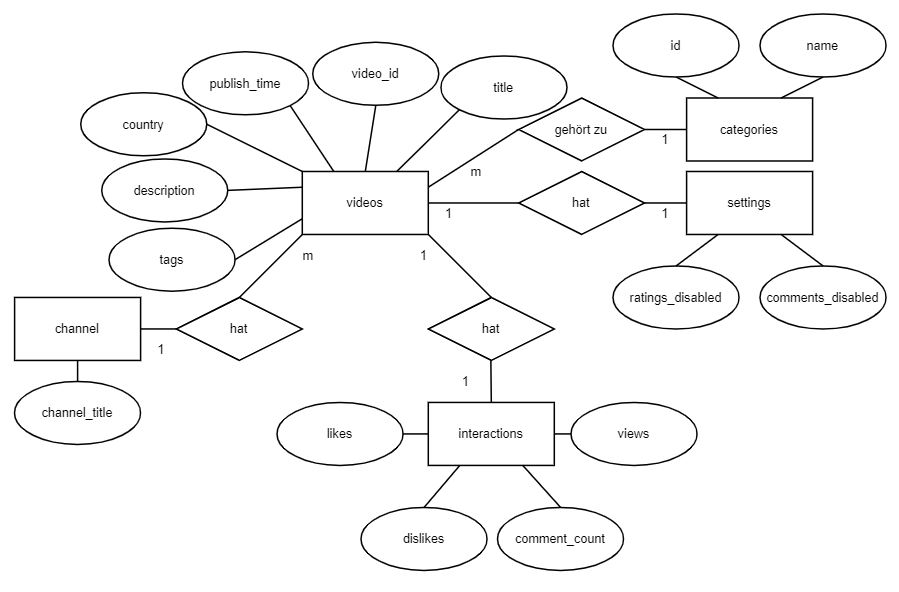
\includegraphics[width=15cm]{IMG/e.jpg}
\caption[Modellierung UML]{Modellierung UML,\\ Quelle: Autoren}
\label{img: Modellierung Collections}
\end{figure}

Zusätzlich erstellte das Projektteam in Anschluss an den Input zu Dokumentdatenbanken noch ein UML-Diagramm (vgl. Abbildung \ref{img: UML-Diagramm} auf Seite \pageref{img: UML-Diagramm}), um die Collections sowie die Beziehung der untergeordneten Objekte zu modellieren. 

\begin{figure}[h]
\centering
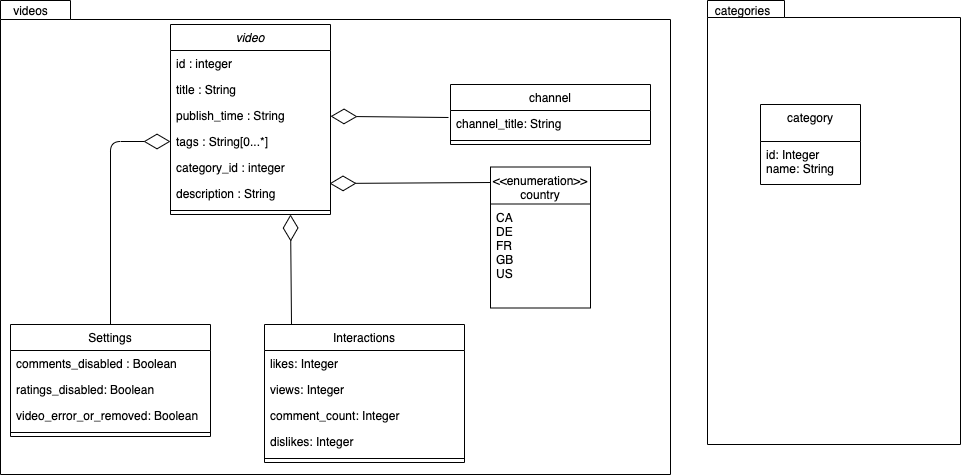
\includegraphics[width=16cm]{IMG/UMLdiagramm.png}
\caption[UML-Diagramm]{UML-Diagramm,\\ Quelle: Autoren}
\label{img: UML-Diagramm}
\end{figure}
\newpage

\subsection{Datenbankschema}\label{Datenbankschema}
Zur Strukturvalidierung des JSON-Dokuments dient ein durch das Projektteam erstelltes JSON-Schema. Dabei erfolgte eine Übersetzung des Datenmodells in das entsprechende Schema. Dieses ist in der folgenden Abbildung (vgl. Abbildung \ref{img: JSON-Schema} auf Seite \pageref{img: JSON-Schema}) ersichtlich.
\begin{figure}
\centering
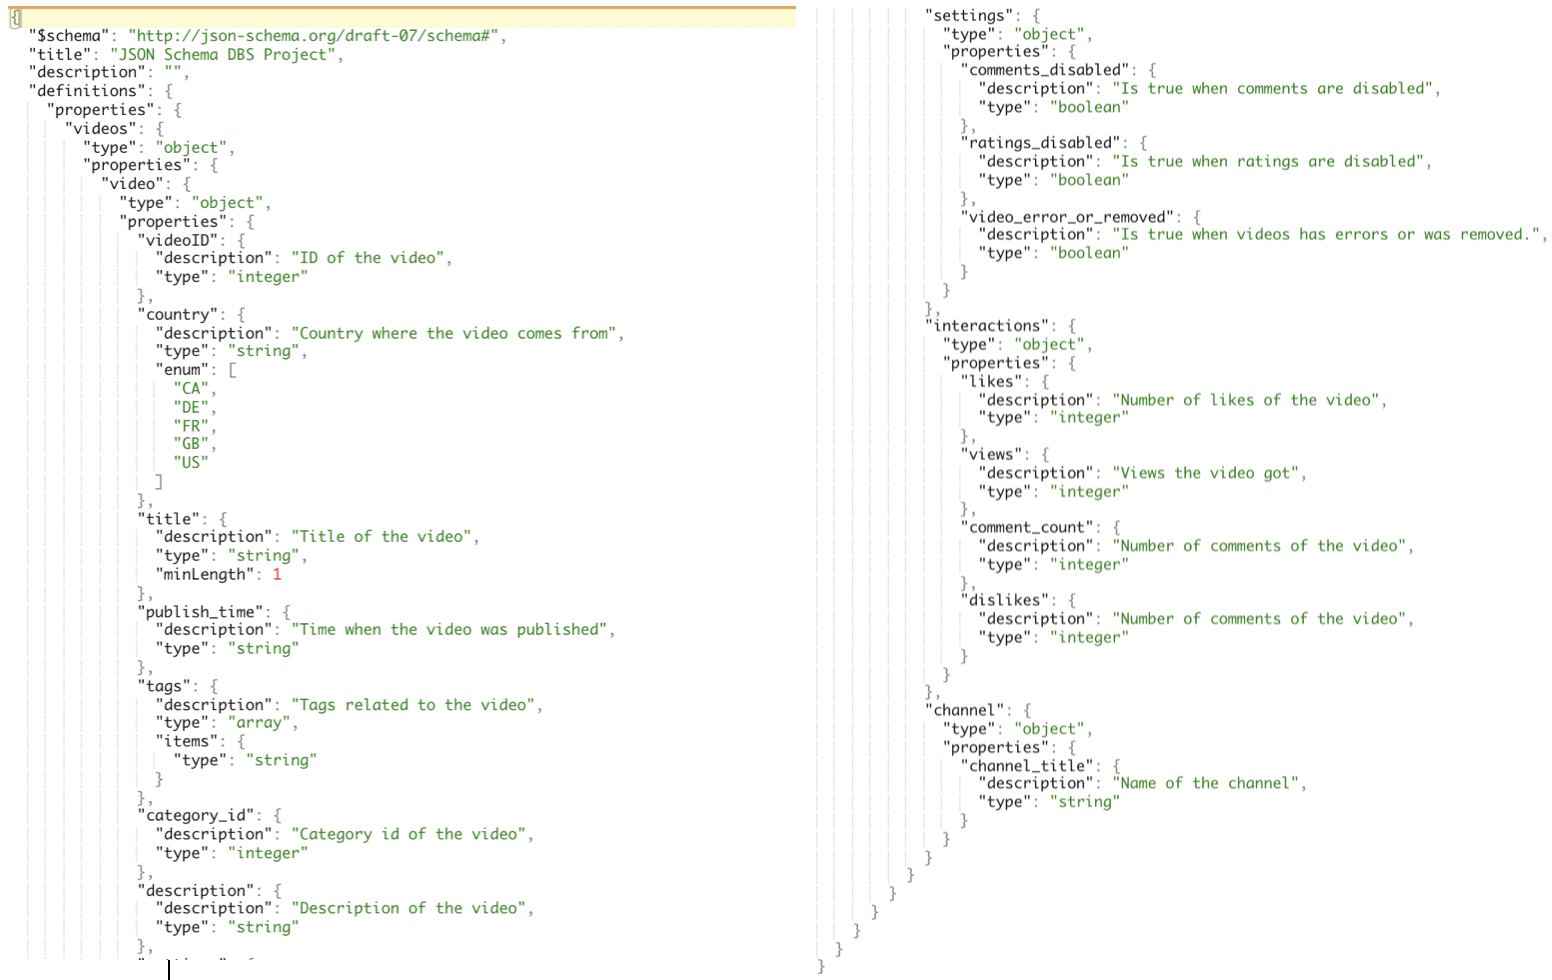
\includegraphics[width=17cm]{IMG/jsonschema.png}
\caption[JSON-Schema]{JSON-Schema,\\ Quelle: Autoren}
\label{img: JSON-Schema}
\end{figure}
\clearpage



%DATENBANKSPRACHE
\section{Datenbanksprache}
Das Projektteam entschied sich, als Abfragesprache Python zu nutzen. Denn Python bietet eine umgängliche API namens Pymongo für die Kommunikation mit MongoDB an.\\
\\
In diesem Abschnitt werden die Abfragen, deren Logik und die eingesetzte Sprache behandelt. Zusätzlich wird gezeigt, wie die Anforderungen gemäss dem Projektauftrag (Selektion, Projektion, Gruppierung, Aggregation etc.) umgesetzt wurden. Die Resultate und Rückgaben der Abfragen werden jedoch erst im Abschnitt Resultate (vgl. Abschnitt \ref{Resultate} auf Seite \pageref{Resultate}) erläutert.

\subsection{Verbindungsaufbau}
Der Verbindungsaufbau zur MongoDB in Python (vgl. Abbildung \ref{fig:Verbindung} auf Seite \pageref{fig:Verbindung}) gestaltet sich einfach. Zunächst gilt es, von Pymongo das Modul \glqq MongoClient\grqq\, zu importieren. Über \glqq MongoClient\grqq\, lässt sich schliesslich unter der Angabe vom Protokoll (mongodb), der IP-Adresse und dem Port ein Client generieren. Von diesem kann schliesslich die Datenbank (hier \glqq DBSFS2020\grqq) sowie die Collection (hier \glqq videos\grqq) angesprochen werden. 
\begin{figure}[h]
\centering
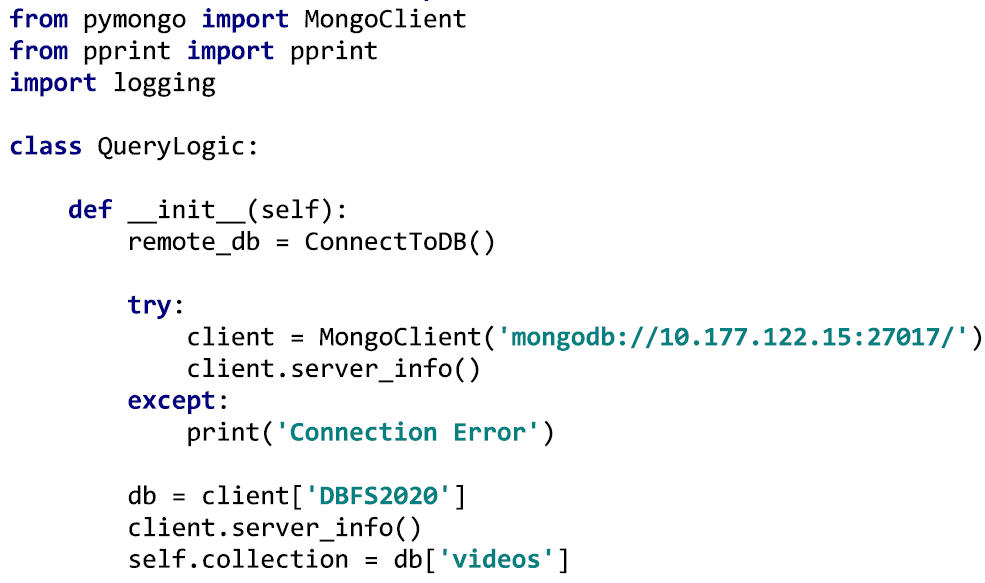
\includegraphics[width=10cm]{IMG/Connect.PNG}
\caption[Aufbau Datenbankverbindung]{Aufbau Datenbankverbindung,\\ Quelle: Autoren} \label{fig:Verbindung}
\end{figure}
\subsection{Join}
In relationalen Datenbanken ist \glqq Join\grqq\, dafür zuständig, Tabellen zusammenzufügen. Im Fall von MongoDB geht es darum, Collections miteinander zu verbinden. In PyMongo wird dies über folgenden Befehl erreicht:
\begin{center}
collection.aggregate([\\\{'\$lookup' : \{...\}\}\\])
\end{center}
Innerhalb der geschweiften Klammern nach \glqq lookup\grqq\, findet schliesslich das Zusammenfügen der Collections statt. Im vorliegenden Projekt finden \glqq Joins\grqq\, ausschliesslich bei der Gruppierung nach Kategorien Anwendung. Denn die durch die Datenquelle (Kaggle) offerierten Daten enthalten lediglich die ID der Kategorie, jedoch nicht deren Namen. Eine ID der Kategorie alleine ist nicht sehr aussagekräftig. Der Anbieter der Daten hat die zugehörigen Namen auf Kaggle leider nicht veröffentlicht. Daher wurden diese im Internet \shortcite{category} gesucht, auf deren Richtigkeit überprüft und schliesslich in einer separaten Collection abgespeichert. Damit ist es möglich, mittels eines \glqq lookup\grqq\, bei der Gruppierung nach Kategorie den Namen der Kategorie anstelle der ID auszugeben.\\
\\
Da das Projekt generell sehr viele Abfragen enthält, wird nicht jede im Quellcode grafisch dargestellt. Daher ist untenstehend lediglich eine davon visualisiert (vgl. Abbildung \ref{fig:Query} auf Seite \pageref{fig:Query}):

\begin{figure}[h]
\centering
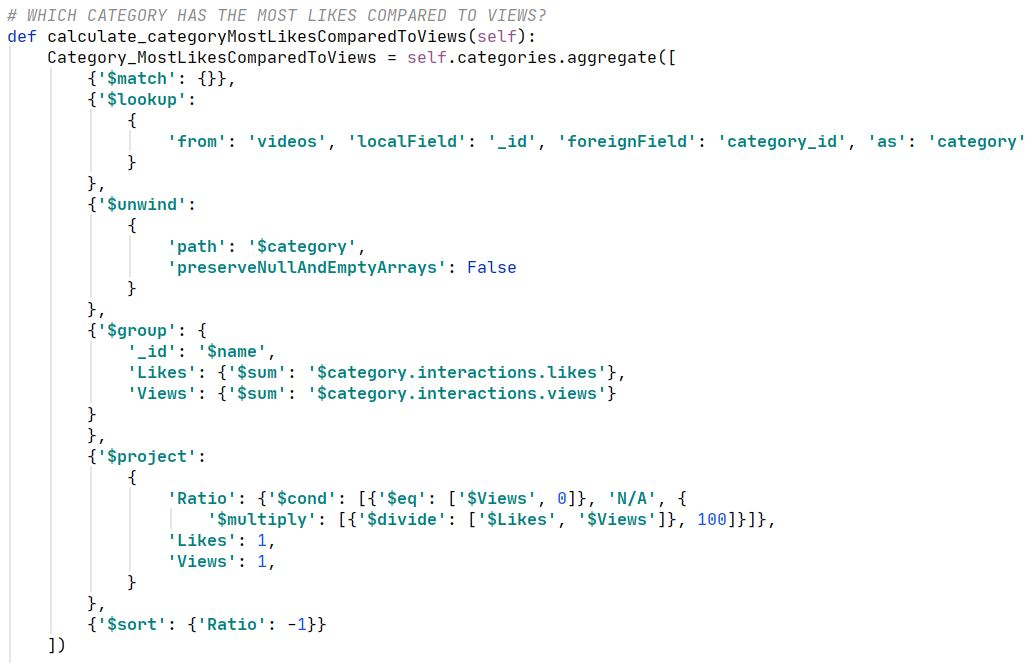
\includegraphics[width=15cm]{IMG/Query.PNG}
\caption[Umfangreiche Abfrage]{Umfangreiche Abfrage,\\ Quelle: Autoren} \label{fig:Query}
\end{figure}

\subsection{Aggregation} \label{Aggregation}
Aggregationen sind dafür da, Auswertungen basierend auf spezifischen Attributen vorzunehmen. Beispiele sind arithmetische Operationen, der Durchschnitt, das Maximum oder das Minimum. Es gibt natürlich noch viele weitere. Die folgende Auflistung (vgl. Tabelle \ref{Aggregation: Beispiele} auf Seite \pageref{Aggregation: Beispiele}) zeigt, wie einige solcher Aggregationen in PyMongo aussehen.
%Aggregationen
\begin{table}[htbp]
\centering
\begin{tabular}{ll}
\hline
Befehl & Bedeutung\\
\hline\\
\$sum & Summe \\
\hline\\
\$divide & Division \\
\hline\\
\$multiply & Multiplikation \\
\hline\\
\$avg & Durchschnitt \\
\hline\\
\$max & Maximum \\
\hline\\
etc. & ... \\
\hline\\
\end{tabular}
\caption[Aggregation: Beispiele]{Aggregation: Beispiele}
\label{Aggregation: Beispiele}
\end{table}
Aggregationen sind ein wichtiger und grosser Bestandteil der Abfragen im Projekt. In vielen Abfragen ist ein Verhältnis zweier Attribute als Resultat vorgesehen. Verhältnisse sind insofern relevant, dass sie sich besser dazu eignen Resultate zu vergleichen. Möchte man beispielsweise wissen, welche Youtube-Kategorie die meisten Likes hat, ist es ungenau, lediglich das entsprechende Attribut Likes für eine Kategorie aufzusummieren. Angenommen in der einen Kategorie existieren zehn mal so viele Videos wie in einer anderen Kategorie, dann ist vermutlich deren Anzahl Likes auch höher. Deshalb ist ein Verhältnis zwischen den Attributen wichtig. Beispielsweise wäre ein Ansatz, die aufsummierte Anzahl Likes durch die Anzahl existierender Videos in einer Kategorie auszuwerten. Dann wäre die Kennzahl: \glqq Anzahl Likes pro Video innerhalb einer Kategorie\grqq. Durch solche Verhältnisse sind schliesslich Vergleiche von Kategorien viel aussagekräftiger. Die Aggregation ist eine wichtige Funktion, Verhältnisse zu ermitteln. Um auf das Beispiel \glqq Anzahl Likes pro Video innerhalb einer Kategorie\grqq\, zurückzukommen: Hierfür ist zunächst die Summe aller Likes sowie die Menge an Videos innerhalb einer Kategorie zu ermitteln. Dafür eignet sich die Aggregation \glqq \$sum\grqq. Das Verhältnis (prozentual) lässt sich nun noch wie folgt mit einem einfachen Dreisatz berechnen:
\begin{center}
Verhältnis = $\frac{Summe Videos}{Summe Likes}$ $\cdot$ 100
\end{center}
Da der Dreisatz lediglich aus Multiplikations- und Divisions-Operatoren besteht, hält die Aggregations-Funktion auch hierfür eine Lösung bereit. Für die Division ist \glqq \$divide\grqq\, und für die Multiplikation \glqq \$multiply\grqq\, zu verwenden. Ein ähnliches Beispiel ist im Source-Code abgebildet(vgl. Abbildung \ref{fig:Query} auf Seite \pageref{fig:Query}). Dies ist nur ein Beispiel wie eine Aggregation umgesetzt wurde. Das Projekt umfasst jedoch weitaus mehr. Diese sind im Github-Repository ersichtlich \shortcite{github}. 

\subsection{Gruppierung}
Gruppierungen dienen dazu, Attribute mit gleichem Wert zusammenzufassen. In Bezug auf das Projekt wäre dies beispielsweise eine spezifische Kategorie (bsp. \glqq Film \& Animation\grqq). Gruppierungen sind in Pymongo über folgenden Befehl ausführbar:
\begin{center}
collection.aggregate([\\\{'\$group' : \{...\}\}\\])
\end{center}
Auf einer Gruppieren lassen sich gut Aggregationen anwenden (beispielsweise die Summe aller Likes innerhalb einer Kategorie). Gruppierung finden im Projekt primär bei Abfragen auf Kategorien Anwendung. Im abgebildeten Beispiel (vgl. Abbildung \ref{fig:Query} auf Seite \pageref{fig:Query}) ist eine solche Gruppierung ersichtlich. Dort wird zunächst \glqq self.collection.aggregate\grqq\, aufgerufen. Wie bereits beim Abschnitt Aggregation (vgl. Abschnitt \ref{Aggregation} auf Seite \pageref{Aggregation}) gezeigt, ist dies relevant, damit Daten entsprechend aggregiert werden können. Anschliessend folgt die Gruppierung (\glqq \$group\grqq). Darin wird mittels \glqq id\grqq\, bestimmt, welches Attribut für die Gruppierung relevant ist (hier \glqq category\_id\grqq). Im Anschluss folgen die Aggregationen (\glqq Summe der Likes\grqq\, sowie \glqq Summe der Views\grqq) basierend auf der Gruppierung. Anschliessend erfolgt die Projektion der Daten, die im nächsten Abschnitt (vgl. Abschnitt \ref{Projektion} auf Seite \pageref{Projektion}) vertieft wird. Um die Gruppierungen noch genauer zu sehen, wird auch hier ein Einblick in das Github-Repository empfohlen \shortcite{github}.

\subsection{Selektion und Projektion} \label{Projektion}
Im relationalen Datenbankumfeld steht die Selektion für das Auswählen spezifischer Tabellenzeilen, während die Projektion die gewünschten Spalten abbildet. Solche Funktionen lassen sich auch durch Pymongo in den Collections erreichen. \\
\\
Die Projektion erfolgt durch den Befehl \glqq \$project\grqq\, und filtert die gewünschten Attribute aus der Collection. Das Beispiel (vgl. Abbildung \ref{fig:Query} auf Seite \pageref{fig:Query}) zeigt die Projektion auf drei Attribute (Ratio, Likes, Views). Dabei ist auch gut ersichtlich, dass \glqq Ratio\grqq\, neu durch eine Rechnung generiert wird. Die Rechnung besagt grundsätzlich, dass das Verhältnis (prozentual) zwischen \glqq Views\grqq\, und \glqq Likes\grqq\, zu berechnen ist. Falls das Attribut \glqq Views\grqq\, null ist, ist \glqq N/A\grqq\, auszugeben, da \glqq durch-null-teilen\grqq\, mathematisch nicht definiert ist. Man sieht also, dass Attribute auch während der Abfrage dynamisch erstellbar sind.\\
\\
Die Selektion nutzt den Befehl \glqq \$match\grqq\, und gibt lediglich die Objekte aus, die eine bestimmte Bedingung erfüllen. Auch hierfür ist ein Beispiel abgebildet (vgl. Abbildung \ref{fig:Selektion} auf Seite \pageref{fig:Selektion}). Dieser Befehl sagt aus, dass alle Videos auszugeben sind, die in ihren Einstellungen spezifische Werte (true, false) haben. 
\begin{figure}[h]
\centering
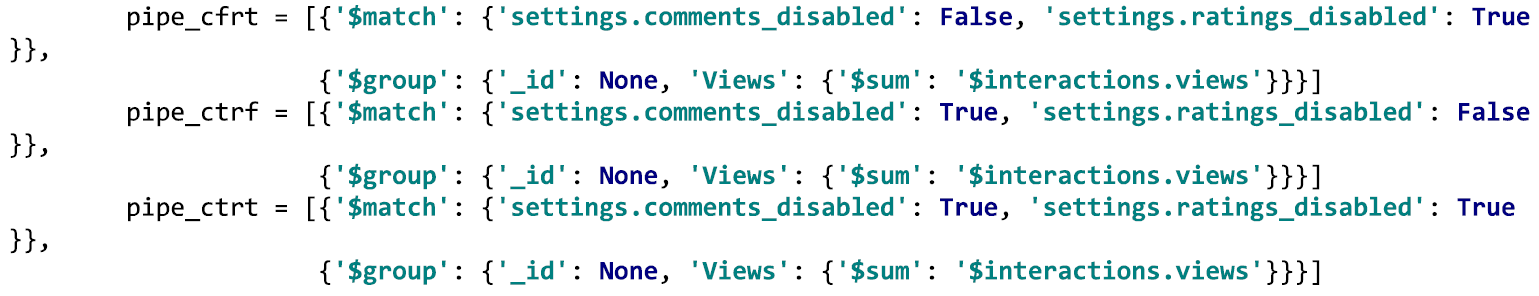
\includegraphics[width=15cm]{IMG/Selektion.PNG}
\caption[Selektion]{Selektion,\\ Quelle: Autoren} \label{fig:Selektion}
\end{figure}


\subsection{Verschachtelung von Queries}
Auch die Verschachtelung der Queries (vgl. Abbildung \ref{fig:Query} auf Seite \pageref{fig:Query}) wurde in den meisten Abfragen genutzt. In der referenzierten Abbildung sieht man beispielsweise, dass innerhalb der Projektion, die entsprechende Ausgabe noch einmal manipuliert wird. Das Resultat verändert sich also insofern, dass von den gruppierten und zusammengefassten Resultaten das prozentuale Verhältnis ermittelt wird. Auch hier ist lediglich ein Beispiel abgebildet. Weitere Verschachtelungen sind ebenfalls im Github-Repository \shortcite{github} ersichtlich. 
\newpage



%SYSTEMARCHITEKTUR
\section{Systemarchitektur}
\subsection{Aufbau, Installation Server}
Damit alle Teammitglieder mit der Datenbank arbeiten können, wurde hierfür eine Ressource auf dem Enterpriselab bezogen. Die Ressource ist unter folgender URL über SSH erreichbar, wobei über den angegebenen Port auf die Datenbank zugegriffen werden kann: 
\begin{itemize}
\item URL: dbs-f20-iffische.el.eee.intern
\item IP-Adresse: 10.177.122.15
\item Port: 27017
\end{itemize}

Bei der Installation hat sich das Projektteam an die Anleitung der offiziellen Webseite von MongoDB gehalten \shortcite{konfiguration}. Dafür wurde die aktuellste Version \glqq MongoDB 4.2 Community Edition\grqq\, installiert. Nach der erfolgreichen Installation ist der Zugriff auf die Datenbank in der Shell über den Befehl \glqq mongo\grqq\, möglich.\\
\\
Auf die Erstellung und Einrichtung der Datenbankinstanz wird im nächsten Kapitel (vgl. Abschnitt \ref{Quelle und Import} auf Seite \pageref{Quelle und Import}) genauer eingegangen.

\subsection{Quelle und Import der Daten}\label{Quelle und Import}

Wie bereits im Use Case erwähnt, wurde als Quelle ein Datensatz genommen, welcher durch Mitchell Jolly \shortcite{autor} durch ein eigens erstelltes Tool gesammelt wurde. Er stellt diesen \shortcite{dataset} frei zur Verfügung und baut ihn von Zeit zu Zeit mit neuen Daten aus. Dieser Datensatz beinhaltet Daten aus USA, Grossbritannien, Deutschland, Kanada, Frankreich, Russland, Mexiko, Süd-Korea, Japan und Indien und ist insgesamt 514 MB gross. In diesem Projekt hat sich das Projektteam jedoch auf die Daten aus USA, Kanada, Grossbritannien, Deutschland und Frankreich eingeschränkt. Die Daten sind online im CSV-Format erhältlich und enthalten folgende Attribute (vgl. Tabelle \ref{fig: Attribute Video-Collection} auf Seite \pageref{fig: Attribute Video-Collection}):
\begin{table}[htbp]
\centering
\begin{tabular}{llll}
video\_id & trending\_date & title & channel\_title\\
\hline\\
category\_id & publish\_time & tags & views \\
\hline\\
likes & dislikes & comment\_count & thumbnail\_link\\
\hline\\
comments\_disabled & ratings\_disabled & video\_error\_or\_removed & description\\
\hline
\end{tabular}
\caption[Attribute Video-Collection]{Attribute Video-Collection}
\label{fig: Attribute Video-Collection}
\end{table}
\\Um die Daten vom CSV-Format in das JSON-Format zu konvertieren, wurde in Python ein Parser geschrieben. Der Parser wandelt die Daten schemakonform (vgl. Abschnitt \ref{Datenbankschema} auf Seite \pageref{Datenbankschema}) um und speichert diese als JSON-Datei. Auf der MongoDB wurde dann eine Datenbank-Instanz namens \glqq DBSF20\grqq\, mit einer entsprechenden Collection \glqq videos\grqq\, erstellt. Darin wurden die einzelnen Objekte als Dokumente angelegt. Durch Eigenrecherche erstellte das Projektteam zusätzlich eine Collection namens \glqq categories\grqq, um die Kategorie-Namen von Youtube-Videos festzuhalten. 


\subsection{Optimierung Performance}
\subsubsection{Schema}
Eine erste Art, wie sich eine Steigerung aus Sicht der Performance erreichen liesse, wäre das Ändern des vorhandenen Schemas und das Einlesen der Daten. Bisher werden die Videodaten sowie die Kategorien jeweils über ein \glqq \$lookup\grqq\, zusammengeführt. Wie bereits erwähnt, ist das \glqq \$lookup\grqq\, mit einem \glqq Join\grqq\, in SQL zu vergleichen. Es ist bekannt, dass solche Ausführungen generell viel Zeit beanspruchen. Man könnte also Kategorien jeweils direkt in der Collection \glqq videos\grqq\, festhalten. Dadurch müsste man kein \glqq \$lookup\grqq\, mehr durchführen. Auf der Gegenseite hätte man mehr Redundanz und würde mehr Speicher benötigen. Da gemäss Aufgabenstellung jedoch ein \glqq Join\grqq\, verlangt wird, wurde bislang auf die Umstellung auf eine Collection verzichtet. Zudem liegt die Performance aus Sicht des Projektteams aktuell noch im grünen Bereich. Würden mehr Daten verarbeitet werden müssen, sollten die Collections \glqq videos\grqq\, und \glqq categories\grqq\, zusammengeführt werden. Dafür wäre dann aber auch eine Anpassung des Parsers notwendig. 

\subsubsection{Queries}\label{unwind}
Bei den Queries fand das Projektteam eine Lösung, wie diese beim Aufruf von \glqq \$lookup\grqq\, zu optimieren sind. Dafür bietet MongoDB die Aggregation \glqq \$unwind\grqq\, (vgl. Abbildung \ref{fig:Query} auf Seite \pageref{fig:Query}) an. Die Theorie besagt \shortcite{mongoDB}, dass wenn ein \glqq \$unwind\grqq\, unmittelbar auf ein anderes \glqq \$lookup\grqq\, folgt und das \glqq \$unwind\grqq\, auf dem \glqq as-Feld\grqq\, des \glqq \$lookup\grqq\, ausgeführt wird, kann der Optimierer das \glqq \$unwind\grqq\, in der \glqq \$lookup\grqq-Phase zusammenführen. Dadurch wird vermieden, dass grosse Zwischendokumente erstellt werden, welche den Arbeitsspeicher unnötig auslasten. Würde man kein \glqq \$unwind\grqq\, nutzen, müsste man den Ausdruck \glqq \{allowDiskUse: True\}\grqq\, verwenden, was die Performance beeinträchtigen würde. \\
\\
Es gäbe noch weitere Arten, wie sich Queries generell optimieren lassen \shortcite{mongoDB}. Im Kontext der Queries im Projekt konnten diese jedoch nicht genutzt werden. 

\subsubsection{Indexing}
Wie bei SQL ist das Setzen von Indexen auch bei MongoDB möglich \shortcite{optimization}. Dafür gibt es verschiedene Arten wie \glqq Single-Field Index\grqq, \glqq Multikey Index\grqq, \glqq Hashed Indexes\grqq\, etc., die verwendet werden könnten. Wie bereits erwähnt, bewegt sich die aktuelle Zeit für die Datenabfragen in einem akzeptablen Rahmen und bedarf vorerst keiner besonderen Optimierung, zumal in den Queries (vgl. Abschnitt \ref{unwind} auf Seite \pageref{unwind}) bereits eine Verbesserung vorgenommen wurde. Zudem ist der Datensatz nicht statisch, sondern wird hin und wieder ergänzt. Falls das Projekt weiterverfolgt würde, müsste man somit das Indexing mit jedem neuen Datenimport erneut ausführen, was ebenfalls ein wenig Zeit kostet. Deshalb wird vorgeschlagen, Indexe erst zu verwenden, wenn diese aus Performancegründen nötig sind. 

\subsubsection{Hardware}
Eine letzte Möglichkeit, die für die Optimierung der Performance im vorliegenden Projekt in Betracht gezogen wird, sind Anpassungen an den Hardwareressourcen. Dafür wäre eine Kontaktaufnahme mit dem Enterpriselab nötig, da die Daten dort abgespeichert sind. 

\subsection{Sicherheitsaspekte}
Die Realisierung beziehungsweise Umsetzung der Sicherheitsaspekte ist nicht Bestandteil dieses Projektes und wurde auch nicht verlangt. Trotzdem hat sich das Projektteam darüber Gedanken gemacht und in der Theorie ein Konzept erarbeitet sowie einiges davon umgesetzt. In diesem Kapitel wird auf die einzelnen Sicherheitskomponenten eingegangen und erläutert, wie diese effektiv umgesetzt oder in der Theorie konzeptionell erarbeitet wurden. Wichtig zu erwähnen ist, dass der Zugriff auf die Daten eher uninteressant für einen Angreifer ist, da diese von einer öffentlichen Datenquelle bezogen wurden.

\subsubsection{Netzwerk}
Die Datenbank wurde auf einer VM installiert, welche sich in der DMZ des Enterpriselabs der Hochschule Luzern befindet. Somit ist diese bis und mit dem OSI Layer 6 bereits abgedeckt. Die Verantwortung dafür hat das Enterpriselab. Aus diesem Grund wurden auf der Netzwerkebene keine weiteren Einschränkungen eingerichtet. Jeder, der sich in der DMZ befindet, hat Zugriff auf diesen. Des Weiteren läuft der MongoDB-Server auf dem Standard-Port 27017. Dies könnte man noch anpassen, da dieser Port bei einem Angriff normalerweise als erstes gewählt wird. \\
\\
Ziel des Projektes ist es, die evaluierten Daten der Öffentlichkeit zur Verfügung zu stellen. Um dies zu ermöglichen, müsste der Server ausserhalb der DMZ zugänglich sein. Hierfür würde man bei einem entsprechenden Cloud-Anbieter (Platform as a Service) eine Dienstleistung beziehen, um den Datenbankserver darauf zu betreiben.

\subsubsection{Usermanagement}
Auf dem Server wurde kein Usermanagement realisiert. Darauf wurde aus zeitlichen Gründen verzichtet. In der Theorie wurde jedoch folgendes überlegt: Für alle Besucher des Webauftrittes, die Abfragen auf der Datenbank machen wollen, besteht lediglich ein lesender Zugriff (kein Delete, Update, etc.). Die wäre über einen entsprechenden User möglich. Rechte für Änderungen werden lediglich einem Administratorkonto erteilt. Mit dem Administratorkonto könnte man sich hingegen nicht über den Webauftritt einloggen, sondern lediglich über die zur Verfügung gestellte Plattform, auf dem sich der Datenbankserver befindet (beispielsweise über SSH). Auf die technischen Aspekte im OSI Layer 7 wird im nächsten Kapitel weiter eingegangen. 

\subsubsection{Applicationlayer}
Da bis zum OSI Layer 6 durch den Plattformbetreiber alles abgedeckt ist, bleibt nur noch das letzte OSI Layer übrig. Wie bereits erwähnt, besteht über den Webauftritt lediglich ein lesender Zugriff auf die Datenbank. Es steht somit kein Loginfenster zur Verfügung. Die gewünschten Datenbankabfragen werden beim Webauftritt über Dropdown-Menüs als Auswahl zur Verfügung gestellt. Auch hier wird auf ein Eingabefeld verzichtet. Nichtsdestotrotz wäre es aber auch hier noch möglich den HTTP-Header zu verändern und so weiteren Schadcode einzufügen. Da aber im Backend lediglich bestimmte Funktionen (ohne Parameterübergabe) aufgerufen werden, besteht hierfür keine Gefahr für eine Injection. Bei der Recherche über Injections auf MongoDB-Servern stellte sich des Weiteren heraus, dass sogenannte SQL-Injections in dieser Technologie kein Problem darstellen, da die Queries als JSON-Objekte und nicht als Strings angelegt werden. Das bedeutet aber nicht, dass die MongoDB immun gegen solche Arten von Angriffen ist. Es ist immer noch möglich, beispielsweise JavaScript-Code einzuschleusen und auszuführen. Auch hierfür kann man auf dem Server einfach JavaScript ausschalten. Dies wäre in diesem Projekt möglich, da im Backend nicht damit gearbeitet wird.
\newpage



%RESULTATE
\section{Resultate}\label{Resultate}
Die Resultate sind in zwei Abschnitte gegliedert. Zunächst wird der Mehrwert für den Nutzer (Youtuber) aufgezeigt und mitgeteilt, wie die Webseite genutzt werden kann. Anschliessend folgen noch Auswertungen und Erkenntnisse des Projektteams.
\subsection{User-Story}
Für das Projekt ist grundsätzlich angedacht, dass der Youtuber die Möglichkeit hat, seinen Account über eine durch das Projekt erstellte Webseite zu analysieren. Damit ergibt sich die Möglichkeit, den eigenen Account mit entsprechenden Richtwerten zu vergleichen und Empfehlungen zu erhalten. Die Analyse ist grob in generelle und kategoriespezifische Resultate unterteilt. Bei den generellen Resultaten werden unterschiedlichste Attribute (Views, Likes, Comments etc.) miteinander verglichen und ausgewertet. Dadurch erhält man eine Übersicht über die gesamte Spannweite. Kategoriespezifisch sind ebenfalls Richtwerte abfragbar. Diese sollen dazu dienen, seinen Account noch konkreter einzuschätzen. Denn zwischen den Kategorien gibt es bei gewissen Kennzahlen teilweise grosse Abweichungen. Kategorienspezifische Abfragen eignen sich aber auch für Einsteiger, die nicht wissen, in welchem Bereich sie Videos machen möchten. Denn gewisse Abfragen (beispielsweise: \glqq welche Kategorie erhält die meisten Views pro Video?\grqq) geben auch Auskunft über die Lukrativität der Kategorien. \\
\\
In der folgenden Aufzählung sind alle Anfragen aufgelistet:
\begin{enumerate}
\item \textbf{Do dislikes have a negative impact on views? (Sorted by Ratio)}
\item \textbf{Do dislikes have a negative impact on views? (Sorted by Views)}
\item \textbf{Do dislikes have a negative impact on views? (Sorted by Dislikes)}
\item \textbf{Are likes relevant for views? (Sorted by Ratio)}
\item \textbf{Are likes relevant for views? (Sorted by Views)}
\item \textbf{Are likes relevant for views? (Sorted by Likes)}
\item \textbf{Are comments relevant for views? (Sorted by Ratio})
\item \textbf{Are comments relevant for views? (Sorted by Views)}
\item \textbf{Are comments relevant for views? (Sorted by Comment)}
\item \textbf{Which category has the most dislikes compared to views?}
\item \textbf{Which category has the most likes compared to views?}
\item \textbf{Which category has the most comments compared to views?}
\item \textbf{Which category gets the most views per video?}
\item \textbf{Which category has the best ratio between likes and dislikes?}
\item \textbf{Which category has the highest amount of uploads?}
\item \textbf{What is the general ratio between likes and dislikes?}
\end{enumerate}
Aus den genannten Fragen ergeben sich nun endlose Szenarien, wie diese nützlich sein können. Nimmt man als Beispiel eine Neueinsteigerin (junge Frau) bei Youtube, die noch nicht weiss, in welchem Bereich sie Videos machen möchte. Daher evaluiert sie mit Abfrage 13, in welcher Kategorie sie statistisch gesehen am meisten Views generiert. Anschliessend prüft sie mit der Abfrage 15, wie hoch die Konkurrenz in den jeweiligen Kategorien ist. Dann entscheidet sie sich für eine Kategorie und beginnt, Videos zu veröffentlichen. Nach einem halben Jahr ist sie entmutigt und überlegt, den Kanal wieder abzubrechen. Sie hat das Gefühl, dass sie sehr viele Dislikes erhält und daher zu viele Leute ihr Videomaterial nicht mögen. Bevor sie sich aber definitiv beschliesst aufzugeben, besucht sie erneut die Webseite und analysiert ihren Account. Zunächst nutzt sie die Abfrage 1, um die Verhältnisse zwischen Dislikes und Views sortiert nach dem Verhältnis zu sehen. Sie merkt, dass sie etwa im Durchschnitt liegt. Das Resultat dürfte also besser sein, ist jedoch lange nicht so schlecht, wie sie es gedacht hat. Sie führt nun noch die Abfrage 2 aus, um zu sehen, was für ein Verhältnis die meistgesehenen Videos haben. Hier macht sich bemerkbar, dass auch solche Videos mit negativer Kritik umgehen müssen, obwohl sie viel Erfolg haben. Nun wird sie langsam erleichtert und ist froh, dass sie die Webseite aufgerufen hat. Ihr wird nun bewusst, dass Zuschauer dazu tendieren, mehr negatives Feedback zu geben, als sie es gedacht hätte. Um sich aber vollständig abzusichern, nutzt sie nun noch Abfrage 10, um kategoriespezifisch die Dislikes zu analysieren. Hier merkt sie nun, dass sie sogar über dem Durchschnitt liegt und ihr Verhältnis daher positiv ist. Sie weiss nun, dass ihre Kategorie verglichen zu anderen mit mehr negativer Kritik rechnen muss. Sie ist nun überzeugt, weiterzumachen. \\
\\
Damit wurde aufgezeigt, wie die Webseite genutzt werden könnte. Dabei liessen sich noch unzählige weitere Szenarien ausdenken. Ein Beispiel wie ein Resultat aussehen könnte, ist im Anhang (vgl. Abbildung \ref{img: Beispiel Auswertung} auf Seite \pageref{img: Beispiel Auswertung}) ersichtlich. Dabei wird die Abfrage 1 visualisiert. 


\subsection{Auswertung Projektteam}
Wie im vorherigen Abschnitt erwähnt, liegt der grosse Mehrwert der Arbeit daran, dass jeder seinen Account selber analysieren kann. Der Youtuber kann somit selbst entscheiden, was für ihn interessant und wichtig ist. Das Projektteam hat die Daten jedoch selbst noch analysiert und dabei einige Erkenntnisse festgehalten. Dafür werden zunächst generelle Resultate und dann kategoriespezifische Resultate aufgezeigt.  

\subsubsection{Generelle Erkenntnisse}
\textbf{Verhältnis von Likes zu Dislikes}\\
Likes und Dislikes sind in der Welt von Social Media Plattformen omnipräsent. Der Tenor hört sich dann oft wie folgt an: Möglichst viele Likes und keine Dislikes. Jedem ist klar, dass das Wunschdenken ist. Interessanter wird es, wenn das Verhältnis von Likes zu Dislikes von allen Videos aus dem Datensatz betrachtet wird. Durchschnittlich sind 5\% (vgl. Abbildung \ref{img: Verhältnis Likes zu Dislikes} auf Seite \pageref{img: Verhältnis Likes zu Dislikes}) aller Bewertungen Dislikes also negativ.
\begin{figure}[h]
	\centering
	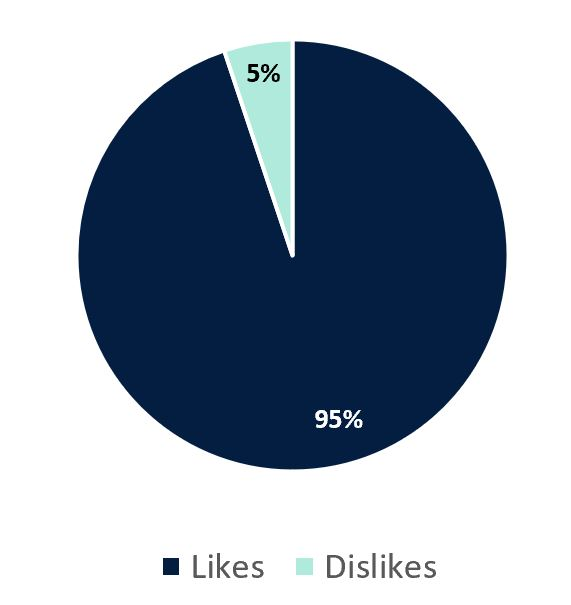
\includegraphics[width=6cm]{IMG/grafik_LikesDislikesRatio.JPG}
	\caption[Verhältnis Likes zu Dislikes]{Verhältnis Likes zu Dislikes,\\ Quelle: Autoren}
	\label{img: Verhältnis Likes zu Dislikes}
\end{figure}

\textbf{Verhältnis von Views zu Dislikes}\\
Man stellt sich des öfteren die Frage, ob die Anzahl Dislikes, nebst den Likes, eine Auswirkung auf die Anzahl Views hat. Diesen Zusammenhang wollte das Projektteam weiter untersuchen und hat dabei die entsprechenden Verhätnisse nach Dislikes, Views und dem Ratio (Verhältnis zwischen Views und Dislikes) sortiert und ausgewertet. Jede Sortierung sagt etwas anderes aus. Bei der Sortierung nach Views sieht man beispielsweise, wie das Verhältnis bei den meistgesehenen Videos ist. Bei der Sortierung nach Ratio erkennt man wiederum, was die besten und schlechtesten Verhältnisse sind, während man bei der Sortierung nach Dislikes noch sieht, ob Videos mit vielen Dislikes effektiv auch ein hohes Verhältnis haben oder nicht. Um zusätzlich einen groben Richtwert zu erhalten, wurde jeweils der Durchschnitt sowie der Median berechnet. Der Median ist sehr tief mit 0.09\% Dislikes pro Anzahl Views (vgl. Abbildung \ref{img:Dislikes pro Views} auf Seite \pageref{img:Dislikes pro Views}). Das heisst, es fallen im Allgemeinen nicht sehr viele Dislikes an.
\begin{figure}[h]
	\centering
	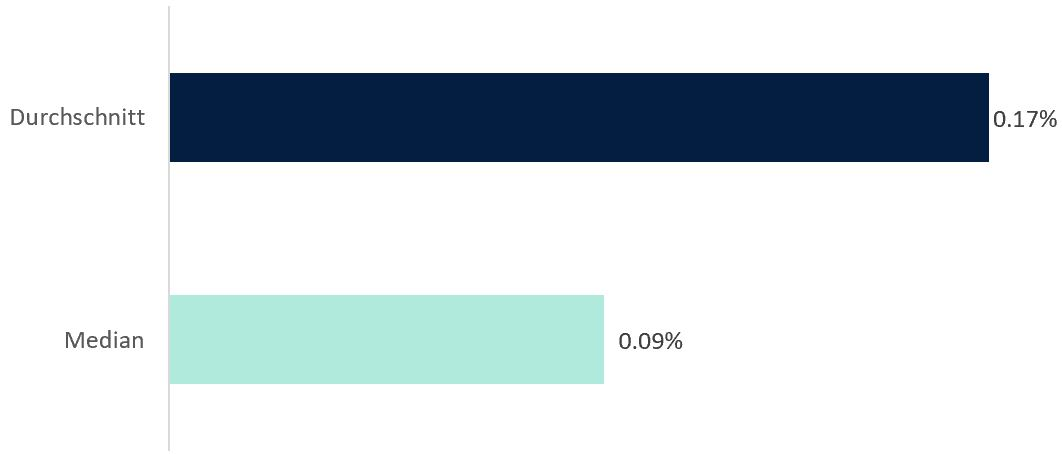
\includegraphics[width=12cm]{IMG/grafik_dislikesviews.JPG}
	\caption[Dislikes pro Views]{Dislikes pro Views,\\ Quelle: Autoren}
	\label{img:Dislikes pro Views}
\end{figure}

\begin{itemize}
\item \textbf{Sortierung nach Ratio:} Hier ist die Spannweite der Erstplatzierten sehr gross. Auf dem ersten Platz landet ein Video mit gerade einmal 3000 Views, während der Viertplatzierte über 600'000 Views hat. Aus diesem Grund ist es hierbei schwierig, eine signifikante Schlussfolgerung zu ziehen.
\item \textbf{Sortierung nach Views:} Videos mit einer hohen Anzahl Views zeigen eine sehr tiefe Anzahl Dislikes auf, was auch zu erwarten war. Wenn ein Video viele Views hat, kann man schlussfolgern, dass das Resultat eher positiv daherkommt. 
\item \textbf{Sortierung nach Dislikes}: Videos mit den höchsten Anzahl Dislikes zeigen einen geringen, aber trotzdem auffäligen Ratio auf. Dieser befindet sich bei allen ca. um 4.3\% wobei die Videos aber auch eine sehr hohe Anzahl Views aufweisen. Sie liegen also massiv über dem Wert des Medians und es handelt sich klar um Ausreisser. 
\end{itemize}

\textbf{Verhältnis von Views zu Likes}\\
Hier wurden die entsprechenden Verhältnisse zwischen Views und Likes berechnet und ebenfalls nach den drei Eigenschaften Views, Likes und Ratio sortiert und ausgewertet. Zudem wurde erneut der Median und Durchschnitt berechnet. Der Median liegt hier bei 2.49\% (vgl. Abbildung \ref{img:Likes pro Views} auf Seite \pageref{img:Likes pro Views}). Man erkennt also sofort, dass mehr Likes als Dislikes anfallen, was auch bereits die Betrachtung des Verhältnisses von Likes zu Dislikes gezeigt hat.
\begin{figure}[h]
	\centering
	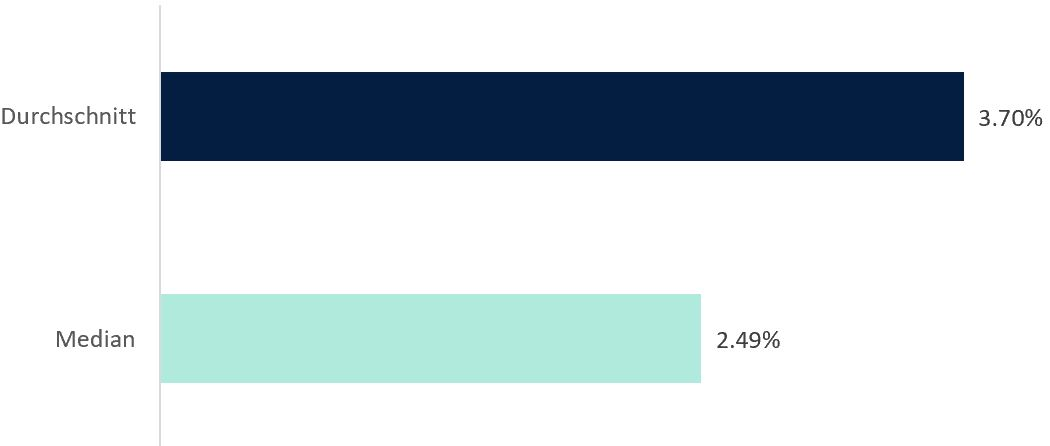
\includegraphics[width=12cm]{IMG/grafik_likesviews.JPG}
	\caption[Likes pro Views]{Likes pro Views,\\ Quelle: Autoren}
	\label{img:Likes pro Views}
\end{figure}

\begin{itemize}
\item \textbf{Sortierung nach Ratio:} Die Spannweite zwischen den Views hierbei ist gross (zwischen 1'000 und 250'000). Aus diesem Grund konnte nicht direkt eine Schlussfolgerung daraus gezogen werden, da sich kein Muster erkennen lässt.
\item \textbf{Sortierung nach Views:} Hier verhalten sich alle Ratios ungefähr gleich (ca. 0.6). Das ist verhältnismässig tief. Bei einer sehr hohen Anzahl Views kann man also nicht zwangsweise schlussfolgern, dass Videos auch eine hohe Anzahl Likes besitzen. 
\item \textbf{Sortierung nach Likes:} Hier schwanken die Ratios zwischen 4 und 5\%. Dieses Verhalten war etwas unerwartet, da die Videos mit den meisten Dislikes auch sehr viele Views hatten. Das ist hier nicht der Fall.  
\end{itemize}
Bei dem Vergleich dieser Sortierungen wurde bestätigt, dass die Anzahl Likes eine positive Auswirkung auf die Anzahl Views haben kann, aber nicht zwingend muss. Die Videos mit den meisten Likes gehören nämlich nicht zu diesen mit den meisten Views. Somit sollte sich ein Youtuber nicht zu sehr auf seine Likes fokussieren, wenn er viele Views als Ziel hat.\\
\\
\textbf{Verhältnis von Anzahl Kommentaren und Views}\\
Hier war nun noch das Verhältnis zwischen den Views und der Anzahl Kommentare relevant. Auch hier wurden die Resultate entsprechend nach Views, Anzahl Kommentaren und den Verhältnissen sortiert. Zudem wurde erneut der Median und der Durchschnitt berechnet, um einen groben Richtwert zu erhalten. In diesem Fall liegt der Median bei 0.31\% (vgl. Abbildung \ref{img:Kommentare pro Views} auf Seite \pageref{img:Kommentare pro Views}) und ist somit um einiges höher als derjenige von den Dislikes pro Views. Es fallen also im Normalfall mehr Kommentare als Dislikes an.

\begin{figure}[h]
	\centering
	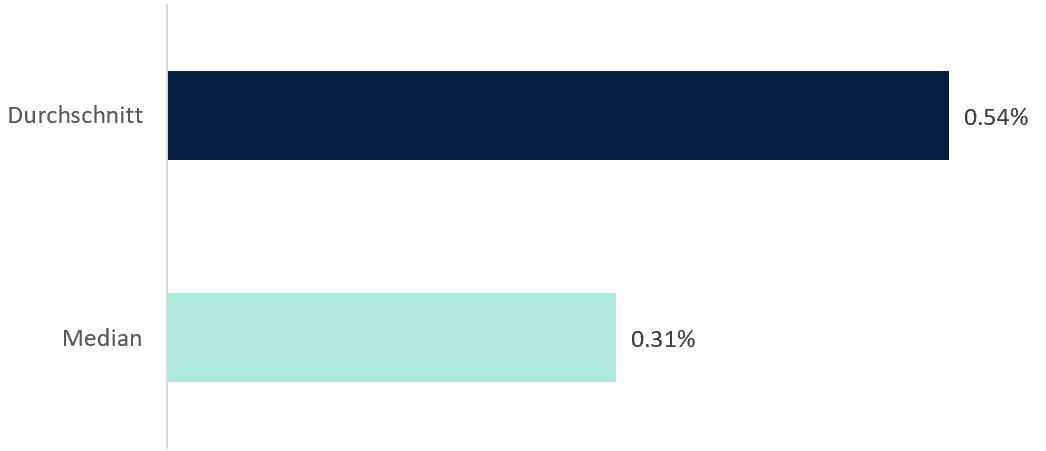
\includegraphics[width=12cm]{IMG/grafik_commentsviews.JPG}
	\caption[Kommentare pro Views]{Kommentare pro Views,\\ Quelle: Autoren}
	\label{img:Kommentare pro Views}
\end{figure}

\begin{itemize}
\item \textbf{Sortierung nach Ratio:} Bei den Videos mit den höchsten Verhältnissen sind erstaunlicherweise nur Videos mit einer Anzahl Views zwischen 20'000 und 46'000 vertreten. Das sind interessanterweise Videos mit sehr wenigen Views.
\item \textbf{Sortierung nach Views:} Bei den Videos mit der höchsten Anzahl Views sind die entsprechenden Verhältnise ebenfalls sehr tief (um die 0.2\%). Hier zeigte sich ebenfalls kein direkter Zusammenhang zwischen der Anzahl Kommentare und der Anzahl Views.
\item \textbf{Sortierung nach Kommentaren:} Hier fielen diejenigen Videos mit einer sehr hohen Anzahl Views auf. Dennoch haben diese aber auch lediglich ein Verhältnis von ca. 3.6\%, was auch hier erstaunlicherweise tief ausfiel. Denn es handelt sich immerhin um die Videos mit den meisten Kommentaren.
\end{itemize}

Es lässt sich hier nicht eindeutig zeigen, dass Kommentare eine sehr wichtige Rollen spielen, um viele Views zu erhalten. Dennoch sind viele Kommentare besser als keine. Dennoch ist es interessant zu erfahren, wie viel Interaktion man mit der Community etwa erreichen kann. 

\subsubsection{Kategorien}
Viele Fragestellungen bezogen sich auf die Kategorien der Videos. Diese wurden durch diverse Abfragen analysiert und ausgewertet.\\
\\
\textbf{Welche Kategorien haben die meisten Likes, Dislikes und Kommentare verglichen mit der Anzahl Views?}\\
Es ist sofort ersichtlich, dass am meisten Likes anfallen und etwas mehr Kommentare als Dislikes (vgl. Abbildung \ref{img:Likes, Dislikes und Kommentare pro Views nach Kategorien} auf Seite \pageref{img:Likes, Dislikes und Kommentare pro Views nach Kategorien}). Dies ist in dieser Form keine Überraschung. Interessanter wird es, wenn die prozentualen Werte etwas genauer betrachtet werden. Hier sticht ganz klar die Kategorie \glqq Nonprofit \& Activism\grqq\, heraus, deren Werte bei allen drei Parametern mit Abstand am höchsten sind. Dies lässt darauf schliessen, dass in dieser Kategorie ein reger und vor allem auch kontroverser Austausch stattfindet. Das konkrete Verhältnis von Likes und Dislikes wird in der nächsten Auswertung noch etwas vertieft. Ansonsten muss jeweils die Kategorie, an der man interessiert ist, betrachtet werden, um die richtigen Schlüsse ziehen zu können.

\begin{figure}[h]
	\centering
	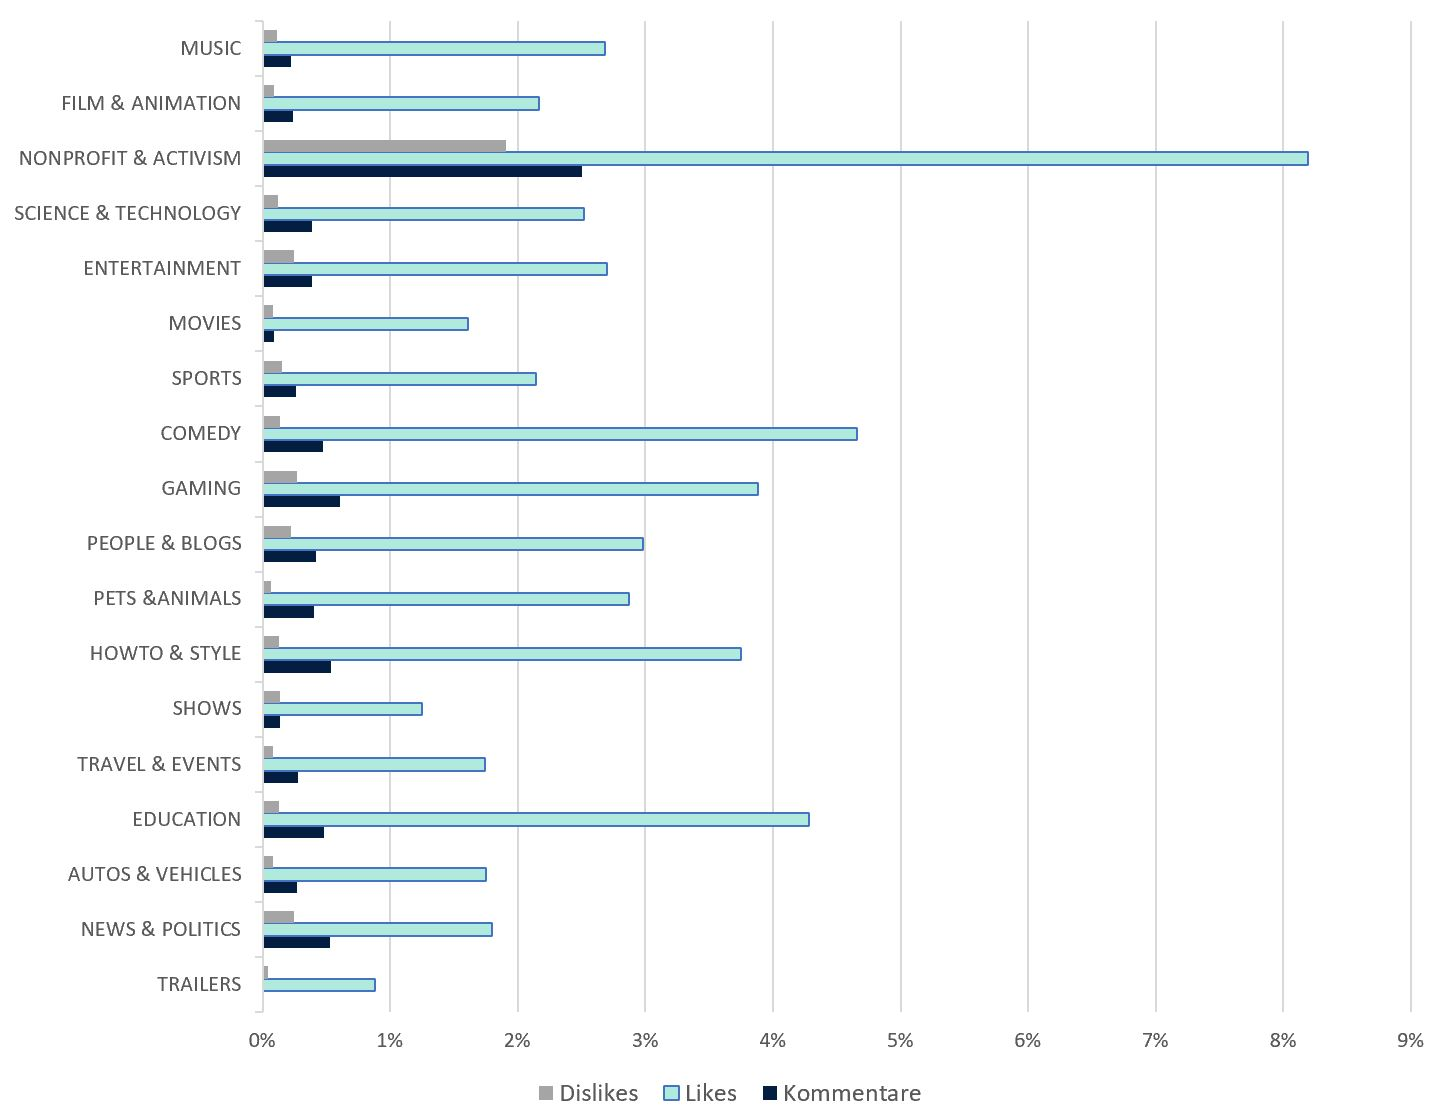
\includegraphics[width=14cm]{IMG/grafik_likesDislikesComments.JPG}
	\caption[Likes, Dislikes und Kommentare pro Views nach Kategorien]{Likes, Dislikes und Kommentare pro Views nach Kategorien,\\ Quelle: Autoren}
	\label{img:Likes, Dislikes und Kommentare pro Views nach Kategorien}
\end{figure}


\textbf{Welche Kategorien haben die höchste Anzahl Views pro Videos?}\\
Die Kategorie \glqq Music\grqq\, belegt hier deutlich den ersten Platz (vgl. Abbildung \ref{img:Views pro Video nach Kategorien} auf Seite \pageref{img:Views pro Video nach Kategorien}). Die restlichen Werte nehmen laufend ab und die Kategorie \glqq Trailers\grqq\, bildet das Schlusslicht mit den wenigsten Views pro Video. Zu beachten ist noch, dass in diesem Datensatz die Kategorie \glqq Music\grqq\, eine sehr hohe Anzahl Videos beinhaltet (lediglich die Kategorie \glqq Entertainment\grqq\, beinhaltet noch mehr Videos). Das heisst, dass die Kategorie enorm viele Views generiert, trotz den sehr vielen Uploads. Weiter unten ist die Uploadmenge der einzelnen Kategorien noch aufgeschlüsselt und erläutert.\\
\\

\begin{figure}[h]
	\centering
	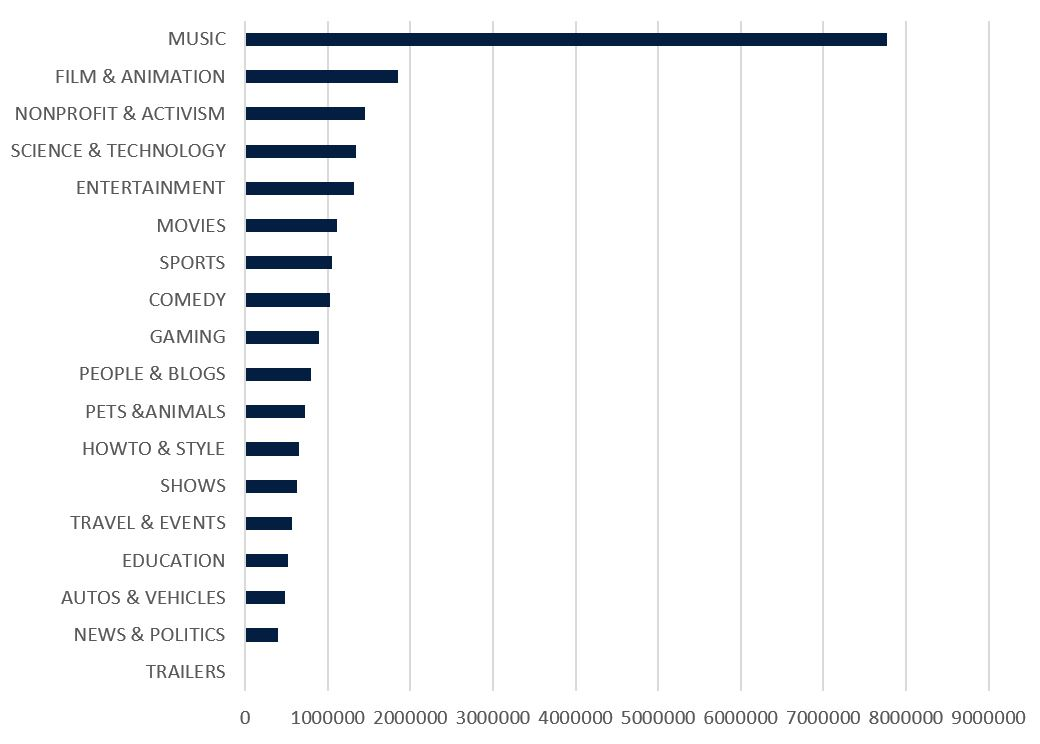
\includegraphics[width=14cm]{IMG/grafik_ViewsProVid.JPG}
	\caption[Views pro Video nach Kategorien]{Views pro Video nach Kategorien,\\ Quelle: Autoren}
	\label{img:Views pro Video nach Kategorien}
\end{figure}


\textbf{Welche Kategorie hat das beste Verhältnis zwischen Likes und Dislikes?}\\
Hier erreicht die Kategorie \glqq Pets and Animals\grqq\, den besten Wert. Nur gerade 2.5\% (vgl. Abbildung \ref{img:Verhältnis Likes zu Dislikes pro Kategorie} auf Seite \pageref{img:Verhältnis Likes zu Dislikes pro Kategorie}) aller Bewertungen sind negativ. Auch hier gilt zu beachten, dass die ersten zehn Kategorien dicht aneinander gereiht sind und sich die Werte nur leicht unterscheiden. Bei der Kategorie \glqq Nonprofit \& Activism\grqq\, sind dann fast ein Viertel der Bewertungen negativ. Spannend ist an dieser Stelle auch noch einen Blick auf die allgemeineren Auswertungen zu werfen. Dort hat sich gezeigt, dass über alle Videos gesehen 5\% aller Bewertungen Dislikes sind. Nun ist gut ersichtlich, dass zwischen den Kategorien doch grosse Unterschiede bestehen.\\
\begin{figure}[h]
	\centering
	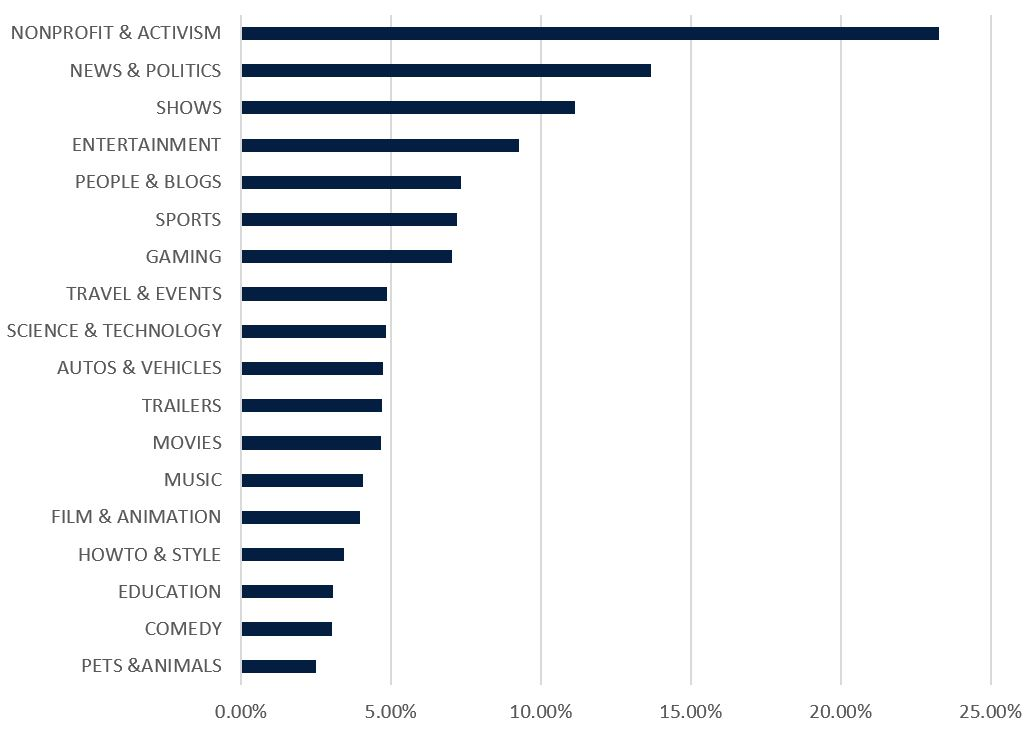
\includegraphics[width=14cm]{IMG/grafik_LikesDislikesKat.JPG}
	\caption[Verhältnis Likes zu Dislikes pro Kategorie]{Verhältnis Likes zu Dislikes pro Kategorie,\\ Quelle: Autoren}
	\label{img:Verhältnis Likes zu Dislikes pro Kategorie}
\end{figure}

\textbf{Unter welcher Kategorie wurde die höchste Anzahl Videos hochgeladen?}\\
Hier hat sich die Kategorie \glqq Entertainment\grqq\, an die Spitze gesetzt (vgl. Abbildung \ref{img: Kategorien sortiert nach Uploadmenge} auf Seite \pageref{img: Kategorien sortiert nach Uploadmenge}), wobei auf dem zweiten Platz die Kategorie \glqq Music\grqq\, ist. Signifikant ist hierbei der rapide Rückgang von der ersten zur zweiten Kategorie. Anschliessend sind die Werte ziemlich gleichmässig abnehmend. Es ist davon auszugehen, dass in Kategorien mit sehr vielen Uploads tendenziell eine grössere Konkurrenzsituation herrscht und es somit schwieriger ist, sich durchzusetzen. 
\begin{figure}[h]
	\centering
	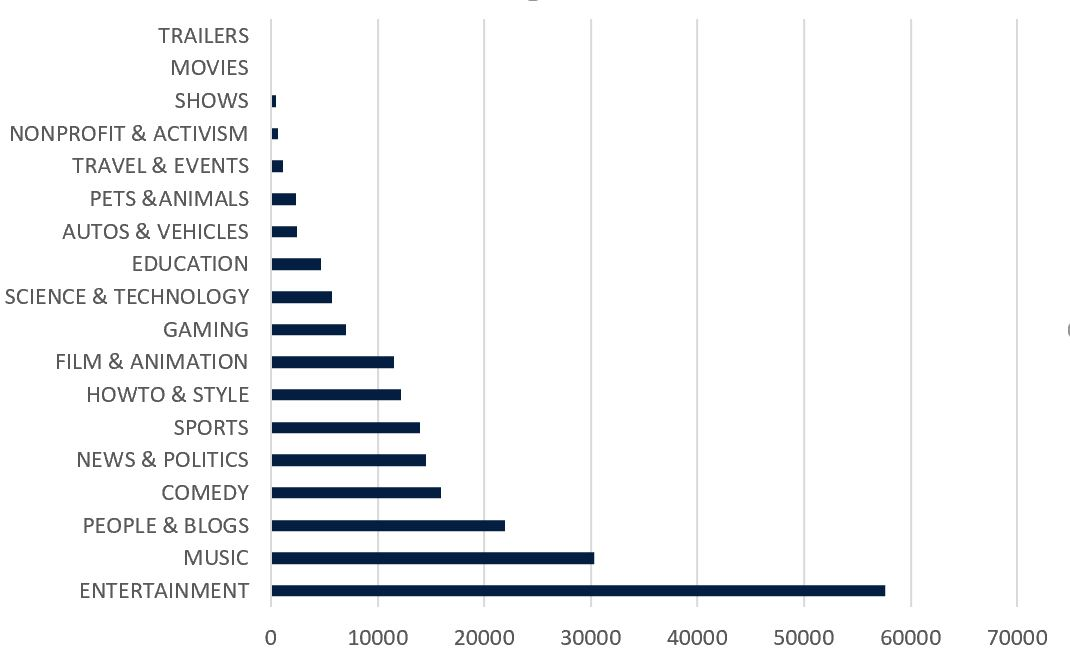
\includegraphics[width=14cm]{IMG/grafik_meisteVideos.JPG}
	\caption[Kategorien sortiert nach Uploadmenge]{Kategorien sortiert nach Uploadmenge,\\ Quelle: Autoren}
	\label{img: Kategorien sortiert nach Uploadmenge}
\end{figure}
\clearpage


\subsection{Zugriff Webseite}
Aus zeitlichen und technischen Gründen hat es für das Deployment der Anwendung des Projekts nicht mehr gereicht. Dennoch soll das Projekt auf der erstellten Webseite für die Bewertung erreichbar sein. Daher wird in den folgenden Schritten erläutert, wie sich die Webseite begutachten lässt:

\begin{itemize}
\item Hierfür ist die Installation von Python nötig. Dazu müssen folgende Packete importiert werden: flask, flask\_wtf, wtforms, json, pymongo
\item Klonen des Githubprojekts mit dem entsprechenden Code. Das Repository ist öffentlich und unter folgendem Link abrufbar:\\
https://github.com/NicoIseli/Datenbanksysteme
\item Verbindungsaufbau mit dem VPN-Service der Hochschule Luzern
\item Start der Klasse Main.py. Die Klasse ist im Projekt unter folgendem Pfad zu finden: Datenbanksysteme/02\_Code
\item Browser öffnen und folgende URL aufrufen: http://localhost:1337
\end{itemize} 
\newpage

%DISKUSSION
\section{Diskussion}
Grundsätzlich besteht bei Kennzahlen, wie jenen von einem YouTube-Kanal, oft die Gefahr, dass diese vollkommen falsch interpretiert werden, da keine Referenz zur Verfügung steht. Durch das vorliegende Projekt wurde nun genau diese Möglichkeit geschaffen, dass jeder seinen Kanal und seine Leistung besser beurteilen kann. \\
\\
Daher ganz klar die Empfehlung: Man sollte sich besser die Zahlen anschauen, statt selbst etwas zu interpretieren. Denn möglicherweise ist jemand gerade in einer Kategorie aktiv, in der es grundsätzlich sehr wenige Likes gibt und die vermeintlich wenigen Likes normal sind. Falls jemand möglichst viele Views pro Video erreichen möchte, dann würde sich die Kategorie \glqq Music\grqq anbieten, die bei Weitem am meisten Views pro Video erreicht. Dabei gilt aber zu beachten, dass in dieser Kategorie auch sehr viele Videos hochgeladen werden. Hat hingegen jemand anderes Interesse an kontroversen Diskussionen, dann wäre die Kategorie \glqq Nonprofit \& Activism\grqq\, eher spannend, da dort sehr viele Kommentare pro Video abgegeben werden und zudem ein hohes Verhältnis von Dislikes zu Likes besteht. Eine weitere sehr wichtige Empfehlung ist, dass die Kategorien auch alleine betrachtet werden sollten, da zwischen ihnen teilweise grosse Unterschiede herrschen. Generell lassen sich aus dem Kapitel \glqq Resultate\grqq\, sehr viele entsprechende Empfehlungen ableiten. Bezüglich den Interaktionen (Likes, Dislikes und Kommentaren) lässt sich festhalten, dass diese eine Rolle spielen, aber nicht einzig für den Erfolg eines Videos verantwortlich sind. Jedoch fallen dabei weitaus am meisten Likes an und daher ist deren Einfluss auch am grössten.
\newpage

%LESSONS LEARNED
\section{Rückblick}
\subsection{Beiträge}
Dieses Projekt hat gesamthaft gesehen einen sehr guten Beitrag an den Lernprozess der einzelnen Teammitglieder geleistet. Die Highlights dabei waren die einzelnen Abfragen, die verwendeten Technologien wie Flask und MongoDB und nicht zuletzt das Zusammenspiel zwischen dem Back- und Frontend. Dieses Zusammenspiel war deutlich aufwändiger als gedacht.

\subsection{Erkentnisse}
Da dieses Projekt mit einer NoSQL-Technologie realisert wurde, musste anfangs einiges an Wissen selbst angeeignet werden, da beispielsweise die Abfragen, Sprachkonzepte wie auch Optimierungen im Unterricht auf SQL aufgebaut waren oder die Theorie dazu gegen Ende des Semesters kam. Nichtsdestotrotz wurde ein Use Case erarbeitet, das Datenmanagement konzipiert, ein Datenmodell erstellt, ein Schema definiert, möglichst selektive und umfangreiche Abfragen erarbeitet und schlussendlich die Resultate auch visualisiert, um einfacher entsprechende Erkentnisse daraus zu schliessen. 
Betreffend der Realisierung war es teilweise schwierig, die gelernte SQL-Theorie mit einem NoSQL-Lösungsansatz zu praktizieren. Während das Datenmanagement noch sehr verallgemeinert war, fing es bereits bei der Datenmodellierung an, genauere Gedanken zu fassen, wie das Ganze in NoSQL realisiert werden soll. Da mit Dokumenten und nicht mit Tabellen gearbeitet wurde, musste man dabei etwas umdenken. Die Dokumentendatenbanken wurden dann erst in der letzten Vorlesungswoche vorgestellt, wobei einem dann vieles klarer wurde. Bei der Realisierung der Abfragen musste man sich ebenfalls an das Internet wenden. Des Weiteren war die Datenvisualisierung ein Knackpunkt. Da jede Abfrage die Daten unterschiedlich zurückgibt, musste die Visualisierung für jede einzelne Abfrage individuell implementiert werden. Aus diesem Grund wurde die Idee mit Abfragen über Eingabefelder schnell verworfen, da sich die Visualisierung komplexer darstellte als zuerst gedacht.

\subsection{Lessons Learned}
Alle Teammitglieder konnten durch das Projekt sehr viel lernen, da beispielsweise zuvor keines der Mitglieder eine vertiefte Erfahrung mit NoSql-Datenabanken hatte. Durch das Projekt wurde nun das Wissen im Bereich von MongoDB aber auch NoSql-Technologien im Allgemeinen aufgebaut, wovon alle in Zukunft profitieren werden. Nebst der reinen Technologie wurde auch das Fachwissen im Bereich des Datenmanagements und Datenmodellierung vertieft. Speziell Teammitglieder, welche bereits die Blockwoche XML/JSON gemacht haben, brachten in diesem Projekt ihr Wissen über JSON ein und hatten nun die Möglichkeit, dieses im Kontext von der vorliegenden Arbeit weiter zu verbessern. Auf der anderen Seite wurde viel über den entsprechenden Use Case gelernt. Eine der spannendsten Feststellung war, dass sich die Kategorien untereinander sehr stark unterscheiden und es unabdingbar ist, diese für sich separiert anzuschauen, um gute und aussagekräftige Resultate zu erhalten. Wenn nun jemand aus dem Team ein YouTube-Kanal starten möchte, dann stehen durch diese Arbeit alle Informationen bereit, um die Kennzahlen des Kanals besser einzuordnen und damit die richtigen Entscheidungen zu treffen, um erfolgreicher auf YouTube zu sein. Nichtsdestotrotz ist im Nachhinein aufgefallen, dass dieser Use Case doch nicht so einfach zu behandeln war, wie anfangs gedacht. Da während der Vorlesung viel auf SQL aufgebaut war, musste man die entsprechenden Aspekte in der NoSQL-Technologie selbst erarbeiten. Zudem war die Suche nach einem Use Case als auch nach den entsprechenden Daten nicht besonders einfach, da dies in dieser Form noch nie gemacht werden musste. Man stellte sich auch die Frage, ob zuerst nach einem Datensatz gesucht werden soll oder zuerst das Finden eines Use Cases Sinn macht. Ersteres wäre vermutlich die bessere Entscheidung gewesen. Nebst einigen Kritikpunkten ist das Team jedoch sehr zufrieden mit dem vorliegenden Projekt und dankbar für die gemachten Erfahrungen. 
\newpage

\section{Anhang}
\begin{figure}[h]
	\centering
	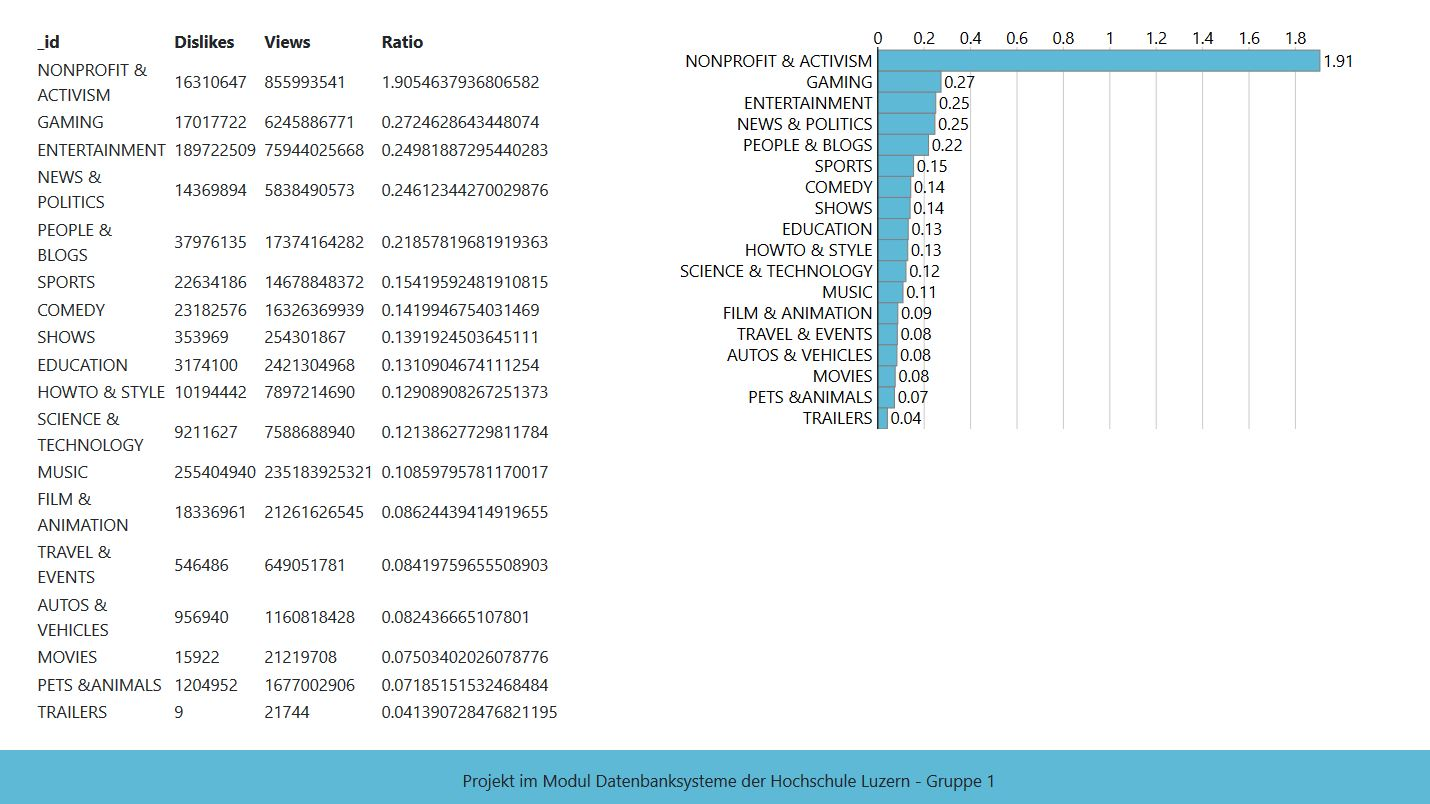
\includegraphics[width=16cm]{IMG/Abfrage1.JPG}
	\caption[Beispiel Auswertung]{Beispiel Auswertung,\\ Quelle: Autoren}
	\label{img: Beispiel Auswertung}
\end{figure}
\newpage



%LITERATURVERZEICHNIS
\bibliographystyle{apacite}
\bibliography{literatur}

\end{document}